\section{Clustering using \acs{optics}}\label{sec:evaluation-OPTICS}
% 3d plots
The algorithm \ac{optics} was applied to data, which was preprocessed according to \autoref{pt:32} and \autoref{pt:eigendocs}.
The clusters from \autoref{fig:optics_cluster} were extracted from the respective reachability plots in \autoref{fig:reachability_plots}.
The three-dimensional plots visualize the first three dimensions of the data and thus, the weights of the first three principal components assigned by the \eigendocs{} algorithm.
By visual inspection and comparison of both plots, it can be seen that the projection by the combination of resizing and \ac{pca} of \autoref{pt:32} scatters the objects further along the $x_2$ axis.
Hence, the distance between the objects is larger and more clusters are identified.
One could argue that the narrow distribution of the objects in the \eigendocs{} plot is due to the fact, 
that the input data encodes not only the visual appearance in terms of page layout but also the size of the document.
Possibly, this could explain why the objects are less scattered along this dimension.

% OPTIC cluster results
\begin{figure}%
    \centering
    \subfloat[\centering Preprocessing according to \autoref{pt:32}.]{{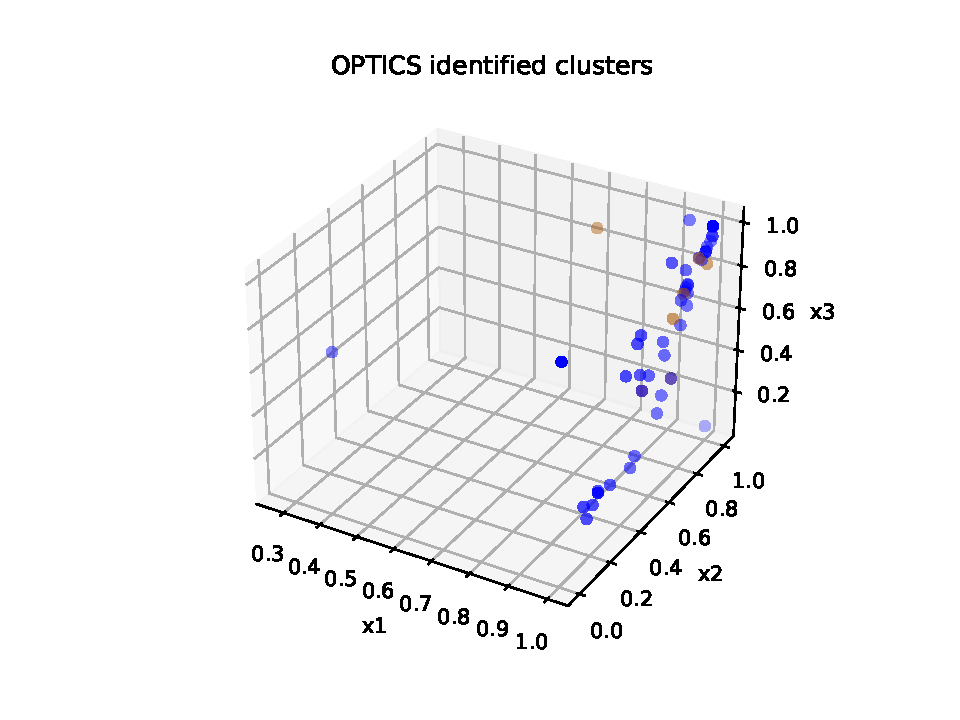
\includegraphics[width=5cm]{images/OPTICS/32x32/OPTICS_cluster_32x32.pdf} }}%
    \qquad
    \subfloat[\centering Preprocessing according to \autoref{pt:eigendocs}.]{{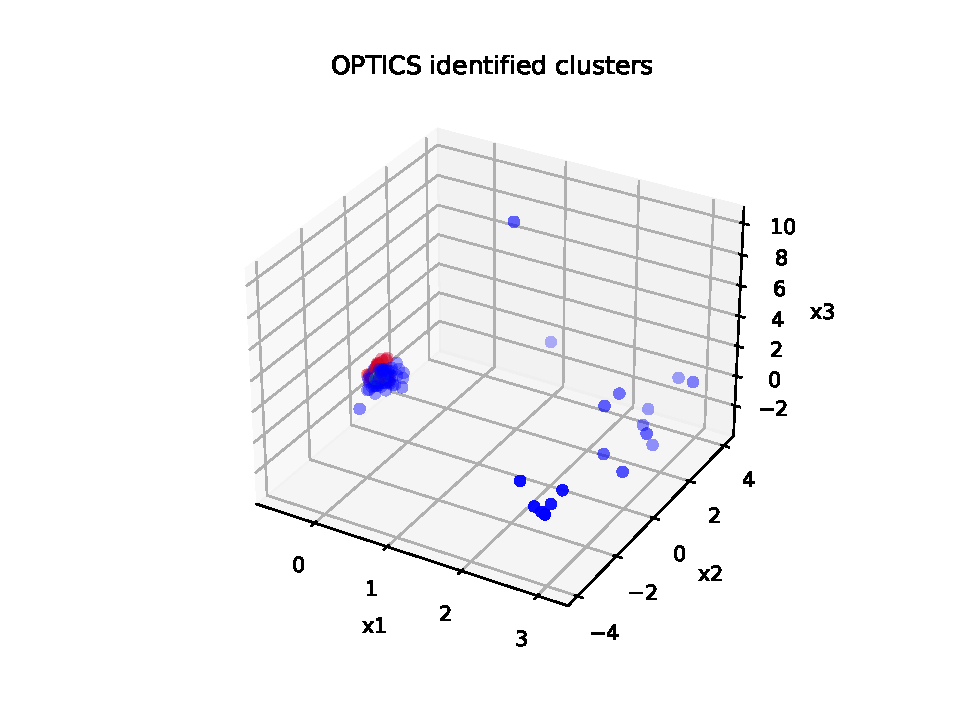
\includegraphics[width=5cm]{images/OPTICS/eigendocs/OPTICS_cluster_eigendocs.pdf} }}%
    \caption[\ac{optics} clusters]{The clusters were extracted from the respective reachability plots in \autoref{fig:reachability_plots} by \ac{optics}.
    The blue points are noise points, whereas any other colour denotes a cluster.}%
    \label{fig:optics_cluster}%
\end{figure}



% cluster content
To analyse the results of the clustering, the content of the clusters was examined.
Since the documents are not labelled, the content of the clusters was analysed by visual inspection.
The content of the clusters is displayed in \autoref{fig:clusters_32x32} and \autoref{fig:clusters_eigendocs_with_noise}.
The yellow images belong to the group identified as noise.
The images preprocessed according to \autoref{pt:32} were partitioned into multiple small and one big cluster.
The \eigendocs{} images' clusters have similar sizes. 
The row of noise images is thus, way longer than the other rows in \autoref{fig:clusters_eigendocs_with_noise}.
Most of the certificates are classified as noise for both approaches.


% 32x32
\begin{figure}[htp] % htp = hier (h), top (t), oder auf einer eigenen Seite (p).
    \centering
    \includegraphics[width=1.05\textwidth]{images/OPTICS/32x32/cluster_content_32x32.pdf}
    \caption[Detailed \ac{optics} clusters using 32x32 greyscale pixels]{The yellow images belong to the group denoted noise.
    Most certificates are classified as noise.
    There is one big cluster and multiple small clusters.
    The images were preprocessed as discussed in \autoref{pt:32} to 32x32 greyscale pixels.
    }
    \label{fig:clusters_32x32}
\end{figure}

% eigendocs with noise
\begin{figure}[htp] % htp = hier (h), top (t), oder auf einer eigenen Seite (p).
    \centering
    \includegraphics[width=1.05\textwidth]{images/OPTICS/eigendocs/cluster_content_incl_noise_Eigendocs.pdf}
    \caption[Detailed \ac{optics} clusters using \eigendocs{}]{Most certificates are classified as noise. The rest of the clusters have similar sizes.
    The images were preprocessed as discussed in \autoref{pt:eigendocs} to 13-dimensional greyscale pixels.
    }
    \label{fig:clusters_eigendocs_with_noise}
\end{figure}


The preprocessing approach used to create the \ac{optics} input for the \databaseName{} database index is \eigendocs{} since it also encodes information about the document size. 

% code
According to \citeauthor{OPTICS2014}, \ac{optics} was developed to improve \ac{dbscan} flaws.
Therefore, \ac{dbscan} is chosen for the cluster method in \lst{lst:optics_model}, since the literature consulted works with \ac{dbscan} as a basis.
In order to reduce calculation complexity the maximum $\varepsilon$ is 10.
The distance between two points to still be considered neighbours is defined after visual inspection of the reachability plot.
Considering the intrinsic structure of the data it is set to $0.5$ to return meaningful clusters.